\section{Przestrzeń $\RR^2$ i $\RR^3$} % wykład 1, 21.02.2019
    
\begin{df}[geometryczna] 
    Wektor definiujemy jako uporządkowaną parę punktów $\langle A,B \rangle$ w przestrzeni $\RR^2$/$\RR^3$ i oznaczam $\overrightarrow{AB}.$
\end{df}
    
Dla wektora $\overrightarrow{AB}$ definiujemy następujące pojęcia:
\begin{itemize}
\item długość --- odległość z punktu $A$ do $B;$
\item kierunek --- kierunek wyznaczany przez prostą przechodzącą przez punkty $A$ i $B;$
\item zwrot --- określamy tylko dla wektorów o tym samym kierunku, dwa wektory mają ten sam zwrot wtedy i tylko wtedy, gdy są skierowane w tą samą stronę. % XD
\end{itemize}
    
Wektory $\overrightarrow{AB}$ i $\overrightarrow{CD}$ uznajemy za równe jeśli mają tą samą długość, kierunek i zwrot.
    
Wektory mogą być swobodne lub zaczepione\footnote{Wektory zaczepione w sumie nas nie interesują, ale warto pamiętać, że
mają one swoje zastowanie, np. w fizyce.}.
    
W algebrze liniowej zazwyczaj utożsamiamy wektor $\overrightarrow{OA}$ z punktem $A$, a za początek układu współrzędnych
przyjmujemy wektor $O=\begin{pmatrix} 0 \\ 0 \end{pmatrix}.$
    
\begin{ft} Dla dowolnego wektora $\overrightarrow{AB}$ zachodzi: $\overrightarrow{AB} = B - A.$ \end{ft}
    
\begin{center}
    \begin{tikzpicture}[scale=1]
        \draw[thick,->] (0,0) -- (5,0) node[anchor=north west] {x};
        \draw[thick,->] (0,0) -- (0,5) node[anchor=south east] {y};
        \filldraw[black] (1,1) circle (1pt) node[anchor=west] {A = $\begin{pmatrix} x_1 \\ y_1\end{pmatrix}$};
        \filldraw[black] (3,4) circle (1pt) node[anchor=east] {$\begin{pmatrix} x_2 \\ y_2\end{pmatrix}$ = B};
        \draw[->] (1,1) -- (3,4);
        \filldraw[black] (4,2.5) circle (0pt) node[anchor=west] {$ \overrightarrow{AB} = 
        \begin{pmatrix}x_2 - x_1 \\ y_2 - y_1\end{pmatrix}$};
    \end{tikzpicture}
\end{center}
    
\begin{df}[algebraiczna]
    Wektor w $\RR^2$ (lub odpowiednio w $\RR^3$) to uporządkowana para (trójka) liczb rzeczywistych.
\end{df}
    
\begin{ozn}
Dla wygody wektory będziemy zapisywać w kolumnie: $\begin{pmatrix} x \\ y\end{pmatrix}$ lub 
$\begin{pmatrix} x \\ y \\ z \end{pmatrix}$
\end{ozn}
    
\begin{minipage}[c]{0.70\textwidth}
Na wektorach w $\RR^2$ definiujemy dwa podstawowe działania:
\begin{itemize}
\item dodawanie wektorów
    \[ \begin{pmatrix} x \\ y\end{pmatrix} + \begin{pmatrix} x' \\ y' \end{pmatrix} =
    \begin{pmatrix} x+x' \\ y + y'\end{pmatrix} \]
\item mnożenie przez skalar
    \[ t \begin{pmatrix} x \\ y\end{pmatrix} = \begin{pmatrix} tx \\ ty \end{pmatrix} \]
\end{itemize}
\end{minipage}%
\begin{minipage}[c]{0.28\textwidth}

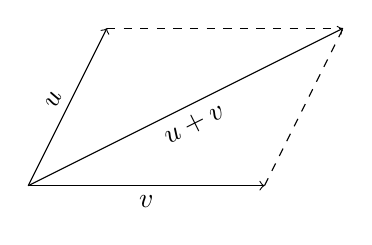
\begin{tikzpicture}
\draw[->] (0,0) -- (1,2) node[midway,sloped,above] {$u$};
\draw[->] (0,0) -- (3,0) node[midway,sloped,below] {$v$};
\draw[dashed] (1,2) -- (4,2);
\draw[dashed] (3,0) -- (4,2);
\draw[->] (0,0) -- (4,2) node[midway,sloped,below] {$u+v$};
\end{tikzpicture} \\
\small{Zasada równoległoboku} \\
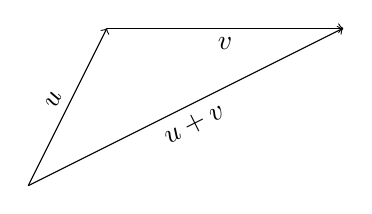
\begin{tikzpicture}
\draw[->] (5,0) -- (6,2) node[midway,sloped,above] {$u$};
\draw[->] (6,2) -- (9,2) node[midway,sloped,below] {$v$};
\draw[->] (5,0) -- (9,2) node[midway,sloped,below] {$u+v$};
\end{tikzpicture} \\ \small{Zasada trójkąta}
\end{minipage}
    
Własności dodawania oraz mnożenia wektorów w $\RR^2 \text{ i } \RR^3$:
\begin{enumerate}[{(}1{)}]
    \item $\forall u, v, w \in \mathbb{R}^2 \quad (u+v)+w = u+(v+w) $
    \item $\forall u, v \in \mathbb{R}^2 \quad u+v = v+u$
    \item $\exists O \in \mathbb{R}^2 \  \forall v \in \mathbb{R}^2 \quad O+v = v+O = v$
    \item $\forall v \in \mathbb{R}^2 \ \exists \text{-} v \in \mathbb{R}^2 \quad v+( \text{-}v) = \text{-} v+v = O$
    \item $\forall u \in \mathbb{R}^2 \ \forall t,s \in \mathbb{R} \quad t(su) = (ts)u$
    \item $\forall u,v \in \mathbb{R}^2 \ \forall t \in \mathbb{R} \quad t(u+v) = tu + tv$ \\ 
          $\forall u \in \mathbb{R}^2 \ \forall t,s  \in
          \mathbb{R} \quad (t+s)u = tu + su$
    \item $\forall u \in \mathbb{R}^2 \quad 1u = u$
\end{enumerate}
    
\begin{ozn} Wektory bazowe będziemy oznaczać jako:
    $e_1 = \begin{pmatrix} 1 \\ 0 \end{pmatrix}$ i $e_2 = \begin{pmatrix} 0 \\ 1\end{pmatrix}$ \end{ozn}
\begin{ft} Każdy wektor w $\RR^2$ zapisuje się jednoznacznie jako kombinacja liniowa wektorów bazowych: $a e_1 + b e_2$ dla pewnych liczb $a$ i $b.$ \end{ft}
    
\begin{df}[algebraiczna]
Iloczynem skalarnym nazywamy funkcję określoną na $\circ\colon\RR^2\times\RR^2\to\RR$ i zadaną wzorem 
\[ \begin{pmatrix} x \\ y\end{pmatrix} \circ \begin{pmatrix} x' \\ y' \end{pmatrix} = xx' + yy' \]
\end{df}
    
Własności iloczynu skalarnego:
\begin{enumerate}[{(}1{)}]
    \item $ \forall u, v \in \RR^2 \ u \circ v = 0 \iff u \perp v$ (przyjmujemy, że wektor $0$ jest prostopadły do każdego wektora)
    \item $ \forall u, v \in \RR^2 \ u \circ v = v \circ u$
    \item $ \forall u, v \in \RR^2 \ \forall t \in \RR \ (tu) \circ v =  t(v \circ u)$
    \item $ \forall u, v, w \in \RR^2 \ u \circ (v + w) = u \circ v + u \circ w$
\end{enumerate}
    
Własności 2, 3, 4 są oczywiste i wynikają wprost z definicji iloczynu skalarnego, natomiast własność 1 najłatwiej jest
pokazać korzystając z definicji geometrycznej iloczynu skalarnego.
    
\begin{df}[geometryczna] 
Iloczyn skalarny można zapisać także w postaci: $$u \circ v = |u||v|\cos\sphericalangle(u, v).$$ \end{df}
    
\begin{tw} Definicja algebraiczna iloczynu skalarnego jest równoważna definicji geometrycznej. \end{tw}
    
\begin{dd}
    Weźmy dowolne dwa wektory $u = ae_1 + be_2$ i $v = a'e_1 + b'e_2$. Łatwo sprawdzić, że obie definicje spełniają
    własności 2, 3 i 4, zatem przekształćmy ich iloczyn skalarny:
    \begin{align*}u \circ v &= (ae_1 + be_2) \circ (a'e_1 + b'e_2) \\
                            &= aa'(e_1 \circ e_1) + ab'(e_1 \circ e_2) + 
                               a'b(e_1 \circ e_2) + bb'(e_2 \circ e_2).
    \end{align*}
    
    Pozostaje pokazać, że zachodzą równości $e_1 \circ e_1 = 1$ oraz $e_1 \circ e_2 = 0$ w obu definicjach. Łatwo. \qed
\end{dd}
    
\begin{tw}[cosinusów]
Niech $a,b,c$ będą długościami boków dowolnego trójkąta i niech $\theta$ będzie kątem naprzeciwko boku o długości $a$, wtedy zachodzi: $c^2 = a^2 + b^2 - 2ab\cos\gamma.$
\end{tw}
    
\begin{dd}
Weźmy dowolne dwa wektory $u,v\in\RR^2$ z kątem $\gamma$ pomiędzy nimi, wtedy wraz z wektorem $w=u-v$ tworzą one trójkąt. Przekształcając: 
\begin{align*} |w|^2 &= w \circ w = (u-v)\circ(u-v) \\ 
                &= u \circ u - u \circ v - v \circ u + v \circ v \\ 
                &= |u|^2 + |v|^2 - 2|u||v|\cos\gamma 
\end{align*}
Kładąc $|u|=a,\ |v|=b, |w|=c$ otrzymujemy tezę. \qed
\end{dd}
    
Analogicznie można zdefiniować powyższe działania i własności dla przestrzeni $\RR^3.$
    
\begin{df}
Wyznacznikiem uporządkowanej pary wektorów $\begin{pmatrix}a \\ b\end{pmatrix}
,\begin{pmatrix} c \\ d \end{pmatrix} $ nazywamy liczbę w postaci: $$\det\begin{pmatrix} a & c \\ b & d\end{pmatrix}=
\begin{vmatrix} a & c \\ b & d \end{vmatrix} = ad - bc.$$
\end{df}
    
Znak wyznacznika informuje nas o orientacji pary wektorów, jeśli jest ujemny, to para wektorów ma orientacje zgodną z
kierunkiem ruchu wskazówek zegara, zaś w przeciwnym przypadku przeciwzegarową.

\begin{center}
    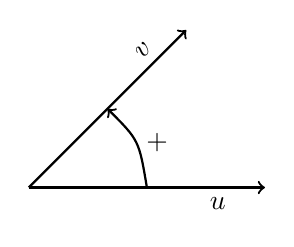
\begin{tikzpicture}
        \draw[thick,->] (0,0) -- (3,0) node[pos=0.8, below] {$u$};
        \draw[thick,->] (0,0) -- (2,2) node[pos=0.8, sloped, above] {$v$};
        \draw[thick,->] (1.5,0) .. controls(1.4, 0.6) ..  (1, 1) node[pos=0.5, right] {$+$};
    \end{tikzpicture}
    \end{center}
\begin{prz}
Para $(u,v)$ jest dodatnio zorientowana.
\end{prz}
    
Wartość bezwzględna wyznacznika równa jest polu równoległoboku rozpinanego przez parę wektorów, skąd możemy otrzymać drugą (równoważną) definicję wyznacznika:

\begin{df}(geometryczna) $\forall u,v\in\RR^2$: $$\det(u,v) = \norm{u}\norm{v}\sin\sphericalangle(u,v).$$ \end{df}
    
\begin{ft}
    Pole dowolnego wielokąta w $\RR^2$ (w którym kolejnie wierzchołki to $v_0,v_1, \dots v_{n-1})$ można wyliczyć za
    pomocą wzoru: 
    \[ \sum_{k=1}^{n-1} \det(v_{k \ mod \ n},v_{k+1 \ mod \ n}) \]
\end{ft}

